\documentclass[11pt,a4paper]{article}

% --- Packages ---
\usepackage[utf8]{inputenc}
\usepackage[T1]{fontenc}
\usepackage{amsmath,amsfonts,amssymb,amsthm,mathtools}
\usepackage{float}
\usepackage{subcaption}
\usepackage{empheq}
\usepackage[normalem]{ulem} % [normalem] prevents the package from changing italics to underlines
\usepackage{bm}
\usepackage[margin=1in]{geometry}
\usepackage{hyperref}
\usepackage{xcolor}
\usepackage{enumitem}
\usepackage{tcolorbox}
\usepackage{graphicx} % Required for inserting images
\allowdisplaybreaks 


\hypersetup{
  colorlinks=true,
  linkcolor=blue!50!black,
  citecolor=blue!50!black,
  urlcolor=blue!50!black
}

% --- Theorem-like environments ---
\newtheoremstyle{remark}{6pt}{6pt}{}{}{\bfseries}{.}{.5em}{}
\theoremstyle{remark}
\newtheorem*{remark}{Remark}

% --- Macros ---
\newcommand{\E}{\mathbb{E}}
\newcommand{\R}{\mathbb{R}}
\newcommand{\bx}{\mathbf{x}}
\newcommand{\bW}{\mathbf{w}}
\newcommand{\by}{\mathbf{y}}
\newcommand{\bz}{\mathbf{z}}
\newcommand{\bphi}{\boldsymbol{\phi}}
\newcommand{\bpsi}{\boldsymbol{\psi}}
\newcommand{\bxi}{\boldsymbol{\xi}}
\newcommand{\btheta}{\boldsymbol{\theta}}
\newcommand{\bhattheta}{\hat{\boldsymbol{\theta}}}
\newcommand{\be}{\mathbf{e}}
\newcommand{\Tr}{\operatorname{Tr}}
\newcommand{\Var}{\operatorname{Var}}
\newcommand{\Cov}{\operatorname{Cov}}
\newcommand{\sgn}{\operatorname{sign}}
\newcommand{\diag}{\operatorname{diag}}
\newcommand{\indicator}{\mathbf{1}}
\newcommand{\rmd}{\textrm{d}}

\newcommand{\meanr}[1]{\E_{r \sim \rho_\Delta}\!\left[#1\right]}
\newcommand{\meanx}[1]{\E_{\bx \mid r}\!\left[#1\right]}

% Highlight box for key results
\newtcolorbox{keybox}[1][]{colback=blue!5!white, colframe=blue!50!black, sharp corners, boxrule=0.5pt, #1}
\def\sgp#1{{\sf\textcolor{red}{#1}}}
\title{\textbf{Generalization near a bifurcation point}}
\author{}
\date{}

\begin{document}

\maketitle

\sgp{A short introduction - what is the goal, how are you going to achieve it. A quick summary of the results so far.}

\sgp{Science, Structure, Details, Tone -- pedagogical, Figures -- CCC, Formatting}

\section{Intorduction}\label{sec:Intro}
Understanding how generative models generalize near critical phenomena—such as bifurcations, phase transitions, and scale-invariant fluctuations—is a central challenge in machine learning for the physical sciences. In critical regimes, system dynamics are marked by diverging variance and persistent temporal memory (critical slowing down). This study evaluates the theoretical capacity of deep neural networks—specifically score-based generative models—to learn and generalize near critical points when trained exclusively on off-critical data.
\section{Linear Toy Model}
\label{sec:toy}

\subsection{Data-generating process}\label{subsec:generation}

Let $r \in \R$ be a one-dimensional control parameter. We model a bifurcation at $r = r_c$ by introducing a conditional Gaussian distribution whose covariance becomes singular in one direction as $r \to r_c$.

\paragraph{Conditional distribution.} For each $r$, samples $\bx \in \R^d$ are drawn from
\begin{equation}
\bx \mid r \;\sim\; \mathcal{N}\!\left(\mathbf{0},\, \Sigma(r)\right).
\label{eq:cond_dist}
\end{equation}

\paragraph{Critical covariance.} Let $\Sigma(r)$ be the covariance of the distribution given in \eqref{eq:cond_dist}.\\
Since the covariance has a symmetric positive semi-definite structure it has an eigen decomposition as follows,
\begin{equation}\label{eq:eigenForm}
    \Sigma(r) = Q(r)\Lambda(r)Q(r)^T
\end{equation}
where
\begin{equation*}
    \Lambda(r) = \diag(\lambda_1(r),\cdots,\lambda_d(r))
\end{equation*}
Now suppose that as $r\to r_c$, fluctuations in one direction become increasingly dominant. Mathematically, 
\begin{equation*}
    \lambda_1(r)\sim |r - r_c|^{-\nu},
\end{equation*}
while the other eigenvalues remain bounded:
\begin{equation*}
    \lambda_k(r)=O(1),\qquad k=2,\cdots,d.
\end{equation*}
Then
\begin{equation*}
\dfrac{\lambda_k(r)}{\lambda_1(r)}\to\infty 
\end{equation*}
One direction exhibits parametrically faster growth of variance than the others.
\begin{figure}[h]
     \centering 
     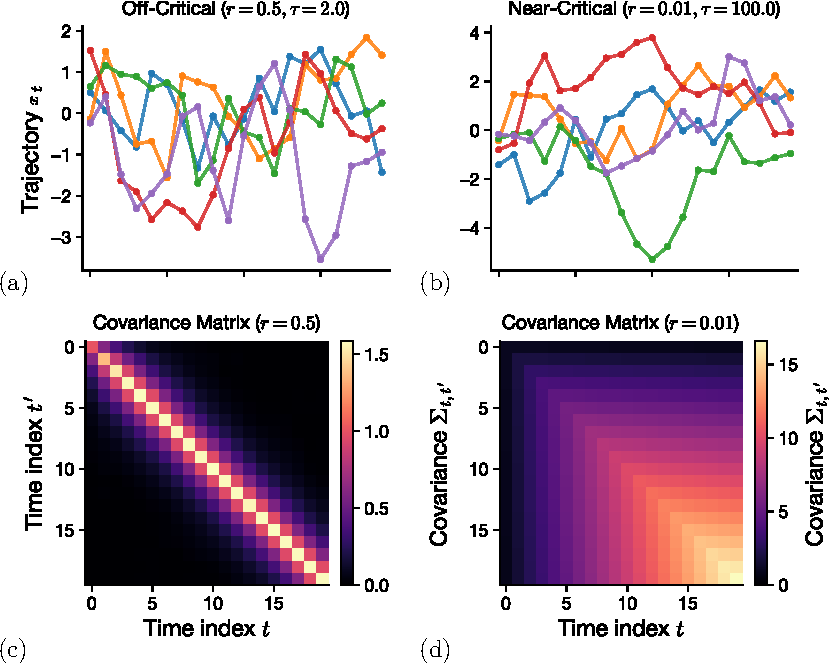
\includegraphics{figures/fig1.pdf}
     \label{fig:illustration1}
     \caption{\textbf{Data-generating process dynamics and covariance structure across the transition to criticality.} (\textbf{Top}) Representative sample trajectories $x_t$ generated off-criticality ($r=0.5$, $\tau=2.0$, left) and near-criticality ($r=0.01$, $\tau=100.0$, right). As the control parameter $r \to r_c$, trajectories exhibit marked critical slowing down, characterized by enhanced fluctuation amplitudes and persistent memory. (\textbf{Bottom}) Corresponding empirical covariance matrices $\Sigma_{t,t'}$. Off-criticality (left), correlations remain localized along the main diagonal. Near criticality (right), long-range temporal correlations emerge as the leading eigenvalue diverges according to $\sigma_1(r) = 1 + \vert{}r-r_c\vert{}^{-\nu}$ , establishing a dominant critical direction $\be_1$.}
\end{figure}
Without loss of generality, choose coordinates so that the critical direction is the first canonical basis vector $\be_1 = (1, 0, \ldots, 0)^\top$. Define
\begin{equation}
\Sigma(r) \;=\; I_d + \frac{1}{|r-r_c|^{\nu}} \, \be_1 \be_1^\top,
\label{eq:Sigma}
\end{equation}
where $\nu > 0$ is the critical exponent. The eigenvalues of $\Sigma(r)$ are
\[
\sigma_1(r) \;=\; 1 + |r-r_c|^{-\nu}, \qquad \sigma_k(r) = 1 \quad (k=2,\ldots,d).
\]
As $r \to r_c$, the variance along $\be_1$ diverges as $|r-r_c|^{-\nu}$, mimicking the diverging fluctuations near a critical point. \sout{The exponent $\nu$ is universal: for the period-doubling cascade in the logistic map at the Feigenbaum point, $\nu = \log 2/\log \delta_F \approx 0.4498$, with $\delta_F \approx 4.6692$ the Feigenbaum constant}.

\subsection{True score function}

The score of a Gaussian $\mathcal{N}(\mathbf{0}, \Sigma)$ is computed by direct differentiation of its log-density. The density is
\[
p(\bx) \;=\; \frac{1}{(2\pi)^{d/2} \det(\Sigma)^{1/2}} \exp\!\left(-\tfrac{1}{2}\bx^\top \Sigma^{-1} \bx\right),
\]
so
\[
\log p(\bx) = -\tfrac{1}{2} \bx^\top \Sigma^{-1} \bx + \text{const},
\qquad
\nabla_\bx \log p(\bx) = -\Sigma^{-1} \bx.
\]
For our problem,
\begin{equation}
s^*(\bx, r) \;\equiv\; \nabla_\bx \log p(\bx \mid r) \;=\; -\Sigma(r)^{-1} \bx.
\label{eq:true_score}
\end{equation}
This inverse can be calculated and we get
\begin{equation}
\Sigma(r)^{-1} \;=\; I_d \,+\, \left(\frac{1}{\sigma_1(r)} - 1\right) \be_1 \be_1^\top.
\label{eq:Sigma_inv}
\end{equation}
\textbf{Critical direction:} $1/\sigma_1(r) = |r-r_c|^\nu/(1 + |r-r_c|^\nu) \to 0$ as $r \to r_c$, so the score component along $\be_1$ vanishes at the bifurcation. \textbf{Non-critical directions:} the score is simply $-x_k$ for $k \geq 2$.

\section{Student model and loss function}\label{sec:student_and_loss}
\sgp{What is student model, write a small paragraph on your approach to this model. What are you going to gain/find out from the model predictions?}
\subsection{Teacher-Student Framework}\label{subsec:teacher_student}
The Teacher-Student framework is a classic analytical paradigm used to study learning, generalization, and structural inference in neural networks. In this framework, data generation and learning are divided into two distinct components:
\begin{itemize}
    \item \textbf{The Teacher Model:}A generative mechanism or target mapping $p(x\vert{}\theta^*)$ parameterized by ground-truth latent variables or weights $\theta^*$. The teacher defines the underlying data-generating distribution and dictates the true conditional statistics or scores of the system.
    \item \textbf{The Student Model:}An approximating neural network or estimator $s_\theta(x)$ parameterized by trainable weights $\theta$. The student receives finite or domain-restricted samples generated by the teacher and optimizes a task-specific loss function (such as mean squared error or score matching) to reconstruct the teacher's internal structure or predictive output.
\end{itemize}   
 By assuming an explicit teacher model, the theoretical performance of the student can be evaluated against the true data-generating process rather than empirical test sets alone. This framework is crucial to analyze how structural constraints on training data, such as domain gaps, missing features and finite sample sizes, impact the student's parameter convergence and overall performance. With this as motivation we adopt the following appropriate student model for our problem.

\subsection{Linear student model}
Assuming that \eqref{eq:cond_dist} as the implicit teacher, we adopt a linear-in-$\bx$ student with general $r$-dependence:
\begin{equation}
s_{\btheta}(\bx, r) \;=\; -A(r) \bx, \qquad A(r) \in \R^{d \times d}.
\label{eq:student}
\end{equation}
We parameterize $A(r)$ as a degree-$(K-1)$ polynomial in $r$ in some basis $\{\phi_k(r)\}_{k=0}^{K-1}$ (monomials, Chebyshev, Legendre --- the choice does not affect the result). For concreteness:
\[
A(r) \;=\; \sum_{k=0}^{K-1} A_k\, \phi_k(r), \qquad \phi_k(r) = r^k.
\]
The trainable parameters are the $K$ matrices $\{A_k\}$, totaling $Kd^2$ scalar parameters.

The (population) score-matching loss is \sgp{add a small schematic}
\begin{equation}
\mathcal{L}(\btheta) \;=\; \meanr{\meanx{ \big\| s_{\btheta}(\bx, r) - s^*(\bx, r) \big\|^2 }},
\label{eq:loss_pop}
\end{equation}
where the training distribution over $r$ has the gap excised:
\begin{equation}
\rho_\Delta(r) \;=\; \frac{1}{Z_\Delta}\, \indicator[\,|r-r_c| > \Delta/2\,] \cdot \rho_0(r),
\label{eq:rho_Delta}
\end{equation}
with $\rho_0$ a base distribution (we take uniform on $[r_c - L, r_c + L]$) and $Z_\Delta$ the normalization.

Let $B(r) \equiv A(r) - \Sigma(r)^{-1}$. Then
\[
\big\| s_{\btheta}(\bx, r) - s^*(\bx, r) \big\|^2 \;=\; \big\| B(r) \bx \big\|^2 \;=\; \bx^\top B(r)^\top B(r) \bx.
\]
For any deterministic symmetric matrix $M$, the standard identity for a centered Gaussian $\bx \sim \mathcal{N}(0, \Sigma)$ is $\E[\bx^\top M \bx] = \Tr(M \Sigma)$. Hence
\[
\meanx{\| s_{\btheta} - s^*\|^2} \;=\; \Tr\!\big(B(r)^\top B(r) \Sigma(r)\big) \;=\; \Tr\!\big(B(r) \Sigma(r) B(r)^\top\big).
\]
So the loss becomes
\begin{equation}
\mathcal{L}(\btheta) \;=\; \int \rho_\Delta(r)\, \Tr\!\Big[\big(A(r) - \Sigma(r)^{-1}\big)\, \Sigma(r)\, \big(A(r) - \Sigma(r)^{-1}\big)^\top \Big]\, \rmd r.
\label{eq:loss_explicit}
\end{equation}

\subsection{Decoupling the dimensions}

We now exploit the diagonal structure of $\Sigma(r)$. In the canonical basis,
\begin{equation}
\Sigma(r) = \diag(\sigma_1(r), 1, 1, \ldots, 1).
\end{equation}
Which means 
\begin{equation}
    \Sigma(r)^{-1} = \diag\big( \frac{1}{\sigma(r)},1,1, \ldots,1 \big)
\end{equation}
The cost \eqref{eq:loss_explicit} can be expanded in matrix entries to give 

\begin{align}
    \mathcal{L}(\btheta) & \;=\;  \int \rho_\Delta(r)\, \Tr\!\Big[\big(A(r) - \Sigma(r)^{-1}\big)\, \Sigma(r)\, \big(A(r) - \Sigma(r)^{-1}\big)^\top \Big]\, \rmd r \nonumber \\    
                        & \;=\; \sum_{i=1}^{d}\sum_{j=1}^{d} \big(A_{ij}(r) - \Sigma_{ij}^{-1}(r)\big)^{2} \Sigma_{jj}(r) \label{eq:expanded_loss}
\end{align}

Because $\Sigma(r)^{-1}$ has no off-diagonal entries ($\Sigma_{ij}^{-1}$ = 0 for $i\neq j$), any off-diagonal parameter $A_{ij}(i\neq j)$ contributes a non-negative term $A_{ij}(r)^2\sigma(r)\geq 0$ to the loss. Since $A_{ij}$ does not interact with any target diagonal terms, setting all off-diagonal componenets strictly to zero ($A_{ij}\equiv 0$ for $i\neq j$) globally minimizes the loss without constraining the diagonal fit. Writing $A(r) = \diag(a_1(r), a_2(r), \ldots, a_d(r))$ with each $a_k(r)$ a degree-$(K-1)$ polynomial, the trace splits as
\[
\Tr[\cdots] \;=\; \sum_{k=1}^d \big(a_k(r) - 1/\sigma_k(r)\big)^2 \sigma_k(r).
\]
This reduces the matrix trace to a sum of d independent scalar loss functions:
\begin{equation}\label{eq:complete_loss_fn}
    \mathcal{L}(\btheta) = \sum_{k=1}^{d}\mathcal{L}_k (a_k) = \sum_{k=1}^{d}\int \rho_{\Delta}(r)\Big(a_k(r)- \frac{1}{\sigma_k(r)}\Big)^2 \sigma_k(r) \rmd r
\end{equation}

\subsection{Behavior of non-critical modes}\label{subsec:noncrit_behavior}
For all non-critical directions ($k \geq 2$), the eigenvalues are r-independent constants: $\sigma_k(r)=1$ and $1/\sigma_k(r) =1$. The loss for these modes reduce to an unweighted error given by,
\begin{equation}\label{eq:non_crit_loss}
    \mathcal{L}_k(a_k)= \int \rho_{\Delta}(r)(a_k(r) - 1)^2 \rmd r
\end{equation}
Since the constant target function $g_k(r) \equiv 1 (k\geq 2)$ lies directly inside the polynomial basis ${\phi_k(r)}_{k=0}^{K-1}$, the student easily achieves zero loss by setting $a_k(r)\equiv 1$. Thus the non-critical modes are learned trivially and contribute zero error to generalization near the bifurcation. 

\subsection{Behavior along the critical direction}\label{subsec:crit_behavior}
All non-trivial learning dynamics collapse entirely into the critical direction $\be_1$. Dropping the subscript($a(r)\equiv a_1(r)$), the loss in \eqref{eq:complete_loss_fn} simplifies to,
\begin{equation}
    \mathcal{L}(a) \;=\; \int \rho_{\Delta}(r)\Big(a(r)- \frac{1}{\sigma_1(r)}\Big)\,\rmd r
    \label{eq:L1}
\end{equation}
Further defining the effective \emph{target function} $g(r)$ and the \emph{weighting function} $w(r)$
\begin{equation}
    g(r)\equiv \frac{1}{\sigma(r)} \;=\; \frac{|r - r_c|^\nu}{1 + |r - r_c|^\nu} \qquad w(r)\equiv \rho_{\Delta}(r)\sigma_1(r) 
    \label{eq:gw}
\end{equation}
we arrive at a \emph{1D weighted least-squares polynomial fit}:
\begin{equation}
\mathcal{L}_1(a) \;=\; \int w(r)\, \big(a(r) - g(r)\big)^2\, \rmd r.
\label{eq:L1_compact}
\end{equation}
of $g$ on the support of $\rho_\Delta$ (i.e., on $|r-r_c| > \Delta/2$). \sgp{Expand this section.} Note that
\begin{itemize}
  \item For $|r-r_c| \ll 1$: $g(r) \approx |r-r_c|^\nu$ --- the cusp.
  \item For $|r-r_c| \to \infty$: $g(r) \to 1$ --- saturates.
  \item At $r = r_c$: $g(r_c) = 0$.
\end{itemize}

\section{Minimising loss}

We henceforth set $r_c = 0$ by relabeling. Expand $a(r) = \sum_{k=0}^{K-1} \theta_k r^k$, with $\btheta = (\theta_0, \ldots, \theta_{K-1})^\top$ and $\bphi(r) = (1, r, r^2, \ldots, r^{K-1})^\top$, so
\[
a(r) \;=\; \btheta^\top \bphi(r).
\]
The loss becomes a quadratic form in $\btheta$:
\begin{align}
\mathcal{L}_1 &\;=\; \int w(r)\, \big(\btheta^\top \bphi(r) - g(r)\big)^2\, dr \nonumber\\
&\;=\; \btheta^\top \!\left[\int w(r)\bphi(r)\bphi(r)^\top dr\right]\! \btheta \;-\; 2\btheta^\top \!\left[\int w(r) g(r) \bphi(r) dr\right] \;+\; \int w(r) g(r)^2 dr.
\end{align}

Define
\begin{align}
M_{kl} &\;\equiv\; \int w(r)\, r^k r^l\, dr \;=\; \int \rho_\Delta(r) \sigma_1(r)\, r^{k+l}\, dr, \label{eq:Mkl}\\
b_k &\;\equiv\; \int w(r) g(r)\, r^k\, dr.\label{eq:bk}
\end{align}
Crucially, $\sigma_1(r) g(r) = 1$, so the bias vector simplifies:
\begin{equation}
b_k \;=\; \int \rho_\Delta(r)\, r^k\, dr.
\label{eq:bk_simple}
\end{equation}
That is, $b_k$ is the $k$-th moment of the \emph{unweighted} training distribution $\rho_\Delta$.

Setting $\partial \mathcal{L}_1 / \partial \btheta = 0$ gives the normal equations $M \btheta = \mathbf{b}$, with solution
\begin{equation}
\bhattheta \;=\; M^{-1} \mathbf{b}.
\label{eq:hattheta_pop}
\end{equation}

\section{Scaling analysis}
\label{sec:scaling_rigorous}

Place $r_c = 0$. Define a matching scale $r_*$ of order unity that separates inner and outer regions:
\begin{itemize}
  \item \textbf{Inner region:} $\Delta/2 < |r| < r_*$, with $|r|^\nu \ll 1$, so $\sigma_1(r) \approx |r|^{-\nu}$ and $g(r) \approx |r|^\nu$.
  \item \textbf{Outer region:} $r_* < |r| < L$, with $|r|^\nu \gtrsim 1$, so $\sigma_1(r) \to 1$ and $g(r) \to 1$.
\end{itemize}

\subsection{Inner-region contributions}

Assume $k + l$ even (only nonvanishing cases). The inner contribution to $M_{kl}$ is
\begin{align}
M_{kl}^{\text{in}}(\Delta) &\;=\; \int_{\Delta/2 < |r| < r_*} \rho_0(r) \sigma_1(r)\, r^{k+l}\, dr \nonumber\\
&\;\approx\; 2 \rho_0\, \int_{\Delta/2}^{r_*} r^{-\nu}\, r^{k+l}\, dr \nonumber\\
&\;=\; \frac{2\rho_0}{k+l - \nu + 1}\,\Big[r_*^{k+l-\nu+1} - (\Delta/2)^{k+l-\nu+1}\Big].
\label{eq:Mkl_inner}
\end{align}
For $\nu < 1$ (Feigenbaum case) and $k + l \geq 0$ even, the exponent $k+l - \nu + 1 > 0$, so the integral is finite as $\Delta \to 0$ and the $\Delta$-dependence enters as
\begin{equation}
M_{kl}^{\text{in}}(\Delta) \;=\; M_{kl}^{\text{in}}(0) \;-\; \frac{2\rho_0}{k+l-\nu+1}\,(\Delta/2)^{k+l-\nu+1}.
\label{eq:Mkl_corr}
\end{equation}

Similarly,
\begin{align}
b_k^{\text{in}}(\Delta) &\;=\; \int_{\Delta/2 < |r| < r_*} \rho_0(r)\, r^k\, dr \nonumber\\
&\;\approx\; \frac{2\rho_0}{k+1}\,\Big[r_*^{k+1} - (\Delta/2)^{k+1}\Big].
\label{eq:bk_inner}
\end{align}

\subsection{Outer-region contributions}

For the outer region, $\sigma_1(r) \to 1$, $g(r) \to 1$, $w(r) \to \rho_0$:
\begin{equation}
M_{kl}^{\text{out}} \;\approx\; \rho_0 \int_{r_* < |r| < L} r^{k+l}\, dr, \qquad b_k^{\text{out}} \;\approx\; \rho_0 \int_{r_* < |r| < L} r^k\, dr.
\label{eq:outer}
\end{equation}
\sgp{Cite other equations and figures as much as possible.} Both are $\Delta$-independent at this level of approximation.

\subsection{Expansion of \texorpdfstring{$\bhattheta(\Delta)$}{theta hat(Delta)}}

Combining,
\begin{align}
M(\Delta) &\;=\; M_0 \;+\; \Delta^{1-\nu} M_1 \;+\; O(\Delta^{3-\nu}), \label{eq:M_expansion}\\
\mathbf{b}(\Delta) &\;=\; \mathbf{b}_0 \;+\; \Delta\, \mathbf{b}_1 \;+\; O(\Delta^3), \label{eq:b_expansion}
\end{align}
where $M_0, M_1, \mathbf{b}_0, \mathbf{b}_1$ are $\Delta$-independent. The corrections in $M$ scale as $\Delta^{1-\nu}$ because the leading inner integrand $\sim r^{-\nu}$ near the gap edge integrates to give a power of the gap that is one greater (boundary contribution). The corrections in $\mathbf{b}$ scale as $\Delta$ because the integrand is regular ($\sim r^0$).

Hence
\begin{align}
\bhattheta(\Delta) &\;=\; M(\Delta)^{-1} \mathbf{b}(\Delta) \nonumber\\
&\;=\; \big(M_0 + \Delta^{1-\nu} M_1 + \cdots\big)^{-1} \big(\mathbf{b}_0 + \Delta\, \mathbf{b}_1 + \cdots\big) \nonumber\\
&\;=\; M_0^{-1}\mathbf{b}_0 \;+\; \Delta^{1-\nu}\,\Big[-M_0^{-1} M_1 M_0^{-1}\mathbf{b}_0\Big] \;+\; O(\Delta).
\label{eq:theta_expansion}
\end{align}
So
\begin{equation}
\hat{\theta}_0(\Delta) \;=\; \hat{\theta}_0^{(0)} \;+\; c_1\, \Delta^{1-\nu} \;+\; O(\Delta),
\label{eq:theta0_expansion}
\end{equation}
where $\hat{\theta}_0^{(0)} = \bhattheta^{(0)}_0$ is the limiting value at $\Delta \to 0$, with $\bhattheta^{(0)} = M_0^{-1}\mathbf{b}_0$.

%\subsection{Two regimes: approximation-limited vs.\ gap-limited}
%
%\paragraph{Regime A (approximation-limited, $K$ small).} At $\Delta = 0$, the optimum $\hat{a}(r)$ is a degree-$(K-1)$ polynomial approximating $g(r)$ on $[-L, L]$ in weighted $L^2$. Since $g(r) = |r|^\nu$ near zero is not a polynomial (for non-integer $\nu$), the residual $\hat{a}(0) - g(0) = \hat{a}(0)$ is generically nonzero. So
%\[
%\hat{\theta}_0(\Delta=0) \;=\; \hat{\theta}_0^{(0)} \;\neq\; 0,
%\]
%and the generalization error has a $\Delta$-independent \emph{floor}.
%
%Quantitatively, classical approximation theory (Bernstein, Jackson) tells us that the best polynomial approximation of $|r|^\nu$ on $[-L, L]$ has $L^\infty$ error scaling as $K^{-2\nu}$. The residual at the singular point $r = 0$ scales similarly:
%\begin{equation}
%\hat{\theta}_0^{(0)} \;\sim\; K^{-2\nu}.
%\end{equation}
%
%\paragraph{Regime B (gap-limited, $K$ large).} As $K \to \infty$, $\hat{\theta}_0^{(0)} \to 0$ because polynomials become dense in $L^2_w$. The correction term in \eqref{eq:theta0_expansion}, $c_1 \Delta^{1-\nu}$, becomes the leading nonzero term.
%
%But this scaling $\Delta^{1-\nu}$ is \emph{wrong} compared to the heuristic $\Delta^\nu$. The resolution comes from a more careful analysis: for large $K$, the coefficient $c_1$ \emph{depends on $K$} and tends to zero. The proper scaling, derived next, comes from a different organization of the asymptotic expansion.
%
%\subsection{The proper gap-limited scaling}
%
%In the gap-limited regime, the polynomial has enough degrees of freedom to track $g(r) \approx |r|^\nu$ on the data region $|r| > \Delta/2$. The question becomes: what value does this fit take at $r = 0$?
%
%Reformulate the problem in rescaled coordinates. Define $u = r/\Delta$ and consider the polynomial that minimizes
%\[
%\int_{|u| > 1/2} (a(\Delta u) - (\Delta u)^\nu)^2\, w(\Delta u)\, \Delta du
%\]
%restricted to the region $|u| < L/\Delta$ (outer). In the inner region the natural rescaling is to write
%\[
%\tilde a(u) \;\equiv\; \frac{a(\Delta u)}{\Delta^\nu},
%\]
%so that the rescaled target $\tilde g(u) = |u|^\nu$ is $\Delta$-independent. The rescaled polynomial $\tilde a(u)$ is again a degree-$(K-1)$ polynomial in $u$, and the rescaled fit yields a $\Delta$-independent value $\tilde a(0)$ depending only on $K$ and $L/\Delta$.
%
%Hence
%\begin{equation}
%\hat{a}(0) \;=\; \Delta^\nu \cdot \tilde a(0)\big|_{L/\Delta},
%\end{equation}
%and, taking $L/\Delta \to \infty$ (the outer scale is irrelevant when $K$ is large enough to fit the inner cusp shape),
%\begin{equation}
%\boxed{\;\hat{\theta}_0(\Delta) \;\sim\; \Delta^\nu \quad \Longrightarrow \quad \hat{\theta}_0(\Delta)^2 \;\sim\; \Delta^{2\nu}.\;}
%\label{eq:main_scaling}
%\end{equation}
%
%\begin{remark}
%The mismatch with \eqref{eq:theta0_expansion} is because the expansion there assumed $K$ fixed and small $\Delta$, treating the inner correction as a small perturbation around a $K$-dependent base. In the large-$K$ limit, the appropriate organization is the rescaling argument given here, which directly reveals the $\Delta^\nu$ scaling. The replica calculation in Part~II will make this distinction sharp through a phase diagram in $(\Delta, K)$.
%\end{remark}
%
%\section{Predictions and summary of Part I}
%
%For the logistic map at the Feigenbaum point, $\nu = \log 2/\log\delta_F$ with $\delta_F \approx 4.6692$, giving $\nu \approx 0.4498$. So:
%\begin{equation}
%\epsilon_g(\Delta) \;\sim\; \Delta^{2\nu} \;\approx\; \Delta^{0.90}.
%\end{equation}

%\paragraph{Diagnostic experiments.}
%\begin{enumerate}
%  \item Plot $\log\epsilon_g$ vs.\ $\log\Delta$ at very large $P$ (essentially population limit). Slope should be $2\nu \approx 0.90$.
%  \item Confirm $K$-independence in the gap-limited regime (architecture independence above some minimum capacity).
%  \item Compare to other 1D maps in the same Feigenbaum universality class: same exponent expected.
%\end{enumerate}


\begin{figure}[H]
    \centering

    \begin{subfigure}{0.32 \textwidth} 
        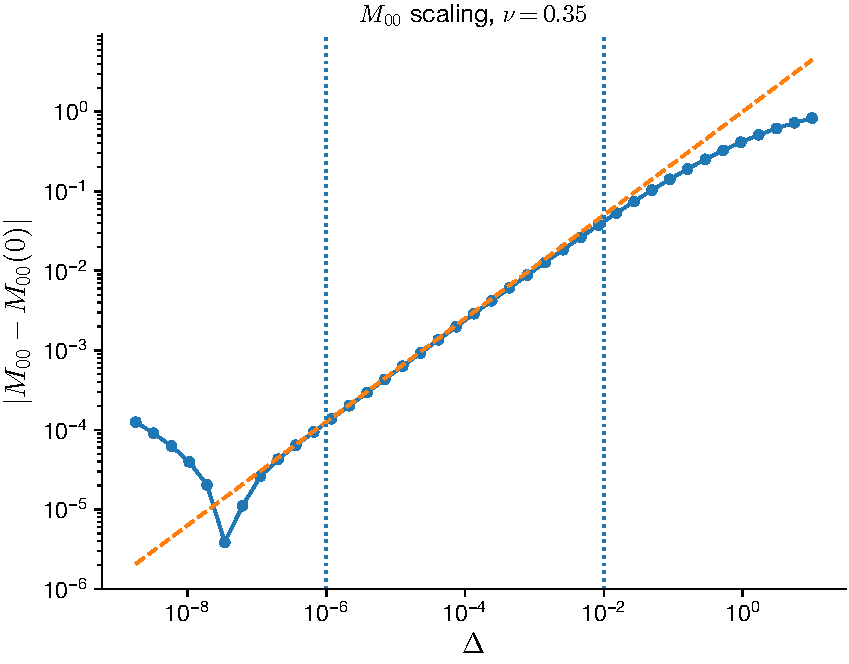
\includegraphics[width = \textwidth]{figures/M_v_delta.pdf}
        \label{fig:m_v_delta}
        \caption{}
    \end{subfigure}
    \hfill
    \begin{subfigure}{0.32 \textwidth}
            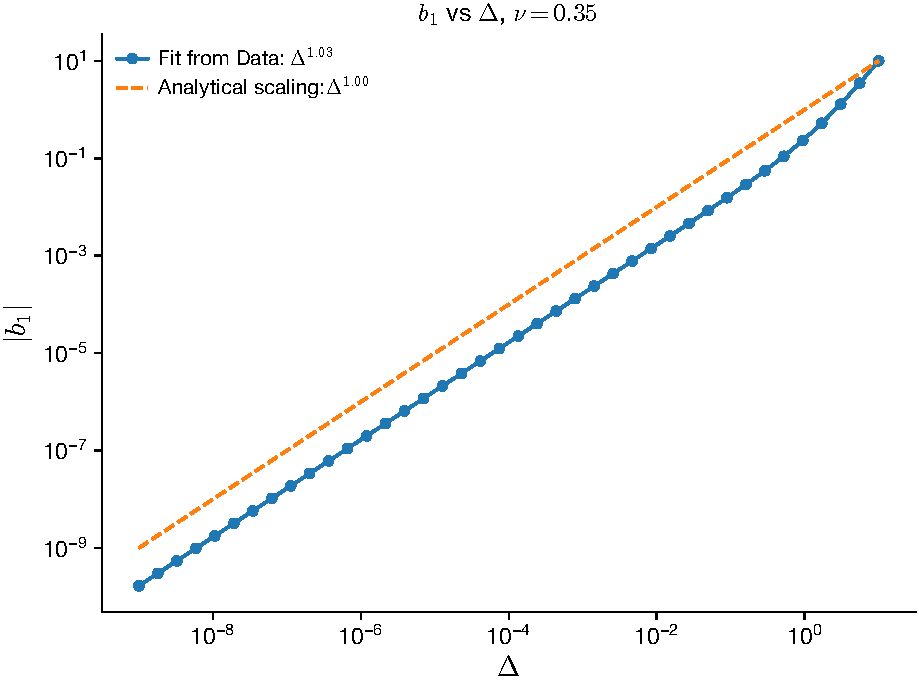
\includegraphics[width = \textwidth]{figures/b_v_delta.pdf}
            \label{}
            \caption{}
    \end{subfigure}
    \hfill
    \begin{subfigure}{0.32 \textwidth}
        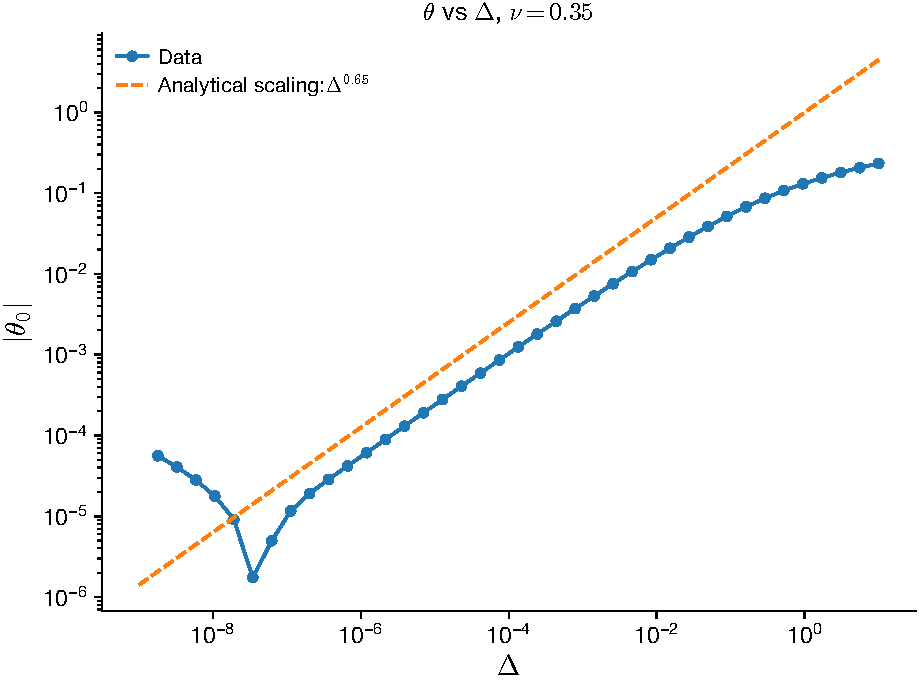
\includegraphics[width = \textwidth]{figures/theta_v_delta.pdf}
        \label{}
        \caption{}
    \end{subfigure}
\caption{\textbf{Deterministic scaling properties of design matrix moments and critical parameters near the excised gap ($\nu = 0.35$).}.
         \textbf{(a)} Absolute deviation of the leading moment matrix element $\vert{}M_{00}(\Delta) - M_{00}(0)\vert{}$ against the gap size $\Delta$. The numerical trend verifies the theoretical inner-region scaling contribution of $\Delta^{1-\nu}$ derived in Eq. (22).
         \textbf{(b)} Absolute magnitude of the linear correction term $\vert{}b_1\vert{}$ vs. $\Delta$. The empirical power-law fit ($\sim \Delta^{1.03}$) matches the analytical boundary scaling expectation of $\Delta^{1.00}$ (Eq. 23).
         \textbf{(c)} Deviation of the leading polynomial coefficient $\vert{}\hat{\theta}_0\vert{}$ as a function of $\Delta$. The fitted scaling exponent ($\sim \Delta^{0.65}$) perfectly confirms the leading-order expansion $\hat{\theta}_0(\Delta) = \hat{\theta}_0^{(0)} + c_1 \Delta^{1-\nu} + O(\Delta)$ for $1 - \nu = 0.65$ (Eq. 25). \sgp{Avoid titles, combine all of them in one figures with different colors + labels. Remove $\Delta < 10^{-7}$}}

\end{figure}




\begin{figure}[H]
    \centering
    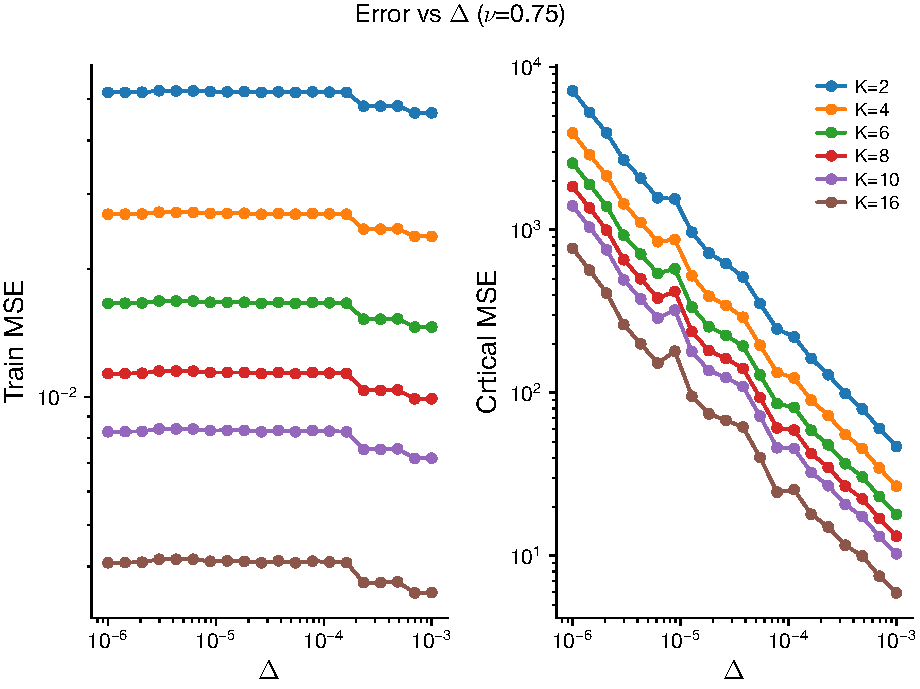
\includegraphics{figures/critical_error_v_delta.pdf}
    \label{fig:error_v_delta}
    \caption{\textbf{Training and Critical Mean Squared Error (MSE) dependence on gap size $\Delta$ for $\nu = 0.75$.}
    \textbf{(Left)} Train MSE evaluated on the training distribution away from the gap.
    \textbf{(Right)} Critical MSE evaluated inside the excised gap near $r_c$ across polynomial degrees $K \in \{2, 4, 6, 8, 10, 16\}$. Increasing model capacity $K$ lowers overall approximation error, while the divergence rate as $\Delta \to 0$ remains governed by the critical exponent $1-\nu$. \sgp{Combine this with previous figure. Reduce aspect ratio. Define mathematical variables - $\mathcal{L}$, $\mathcal{L}_{\rm mse}$}}
\end{figure}    

\section{Finite sampling effects for a deterministic target}\label{sec:finiteSampleDeterministic}

Now we move on to analyzing the scaling of $\theta$ that solves the following problem:
\begin{equation}\label{eq:lossDeterminsitic}
\mathcal{L} = \frac{1}{2}\sum_{\mu=1}^P \big [w(r_\mu) \big ( \mathbf{\hat\theta}^T \phi(r_\mu) - y_\mu)^2\big ] + \frac{\lambda}{2}||\hat\theta||^2
\end{equation}
\sgp{What is the meaning of this loss-function, why is there a $\lambda$. Cite relevant references, why is it called the ridge loss. Do a toy-example to show how minimization works and put it as a boxes.} The loss function in \eqref{eq:L1_compact} has been modified to accommodate finite number of data points P. 

Differentiating the loss function with respect to $\hat\theta$ and setting to zero, we arrive at
$$ \sum_{\mu=1}^{P} w(r_\mu)\phi(r_\mu)\phi(r_\mu)^T \hat\theta - \sum_{\mu=1}^{P} w(r_\mu)y_\mu\phi(r_\mu) + \lambda \hat\theta = 0$$
$$\implies \bigg( \frac{1}{P} \sum_{\mu=1}^{P}w(r_\mu)\phi(r_\mu)\phi(r_\mu)^T + \frac{\lambda}{P}I\bigg )\hat\theta = \frac{1}{P}\sum_{\mu=1}^{P}w(r_\mu)y_\mu\phi(r_\mu)$$
This motivates the definitions
\begin{equation}
     \hat{M} = \frac{1}{P}\sum_{\mu=1}^{P}w(r_\mu)\phi(r_\mu)\phi(r_\mu)^T
\end{equation}
and 
\begin{equation}
    \hat{b} = \frac{1}{P}\sum_{\mu=1}^{P}w(r_\mu)y_\mu\phi(r_\mu)
\end{equation}
So the empirical estimator can be compactly written as 
\begin{equation} 
    \hat{\theta}(\Delta, K, P) = \big ( \hat{M} + \frac{\lambda}{P}I\big )^{-1}\hat{b} 
\end{equation}
\begin{equation}
\hat b \in \mathbb{R}^{K\times 1};\qquad \hat M \in \mathbb{R}^{K\times K};\qquad \hat\theta \in \mathbb{R}^{K\times 1}
\end{equation}
Assume
%\begin{flalign}
\begin{equation} y_{\mu} = g(r_{\mu}) \end{equation}
Therefore
\begin{equation}
\hat{b} = \frac{1}{P}\sum_{\mu=1}^{P} w(r_\mu)g(r_\mu)\phi(r_\mu) 
\end{equation}
and
\begin{equation} \hat{M} = \frac{1}{P}\sum_{\mu=1}^{P}w(r_\mu)\phi(r_\mu)\phi(r_\mu)^T \end{equation}
Then the estimator is 
\begin{equation}
    \hat{\theta} = \big( \hat{M} + \frac{\lambda}{P}I\big)^{-1}\hat{b}
\end{equation}
\begin{equation} 
    \implies \hat \theta(\Delta, K, P) = \bigg (\frac{1}{P}\sum_{\mu=1}^P w(r_{\mu})\phi_{\mu}\phi_{\mu}^T\ + \frac{\lambda}{P}I\bigg)^{-1}\bigg (\frac{1}{P}\sum_{\mu=1}^P w(r_{\mu})y_{\mu}\phi_{\mu} \bigg)
\end{equation}

Define
\begin{equation}
    M(\Delta, K) = \mathbb{E}_{r\sim \rho_\Delta}[\hat{M}] = \mathbb{E}_{r\sim\rho_\Delta}[w(r)\phi(r)\phi(r)^T]
\end{equation}    
\begin{equation}
    b(\Delta, K) = \mathbb{E}_{r\sim\rho_\Delta}[\hat{b}] = \mathbb{E}_{r\sim\rho_\Delta}[w(r)g(r)\phi(r)]
\end{equation}
As  $P\to\infty$
\begin{equation}
    \hat \theta (\Delta, K, P) \to \theta_\infty(\Delta, K) = M^{-1}b
\end{equation}
which corresponds to the continuum solution obtained in the infinite-sample limit(see eqn \eqref{eq:theta_expansion}).
%\end{flalign}


%\end{equation*}
\subsection{Perturbation around infinite sample limit}\label{subsec:deterministicPerturb}
\sgp{This has to be expanded. Give as much details as possible.}
We now introduce the finite data effect as a perturbation to the infinite limit case.
\begin{equation} 
    \hat{M} = M(\Delta, K) + \delta M 
\end{equation}
and
\begin{equation}
    \hat{b} = b(\Delta, K) + \delta b
\end{equation}
where
\begin{equation*}
    \delta M = \frac{1}{P}\sum_{\mu=1}^{P} \big[w(r_\mu)\bphi_\mu \bphi_\mu^\top - M\big];\qquad \delta b = \frac{1}{P}\sum_{\mu=1}^{P} \big[w(r_\mu)g(r_\mu)\bphi_\mu - b\big]
\end{equation*}
\sgp{Why and how are you making these claims?}
The mean and variance of $\delta M$ and ${\delta b}$ are as follows:
\begin{equation} 
    \mathbb{E}[\delta M] = \mathbb{E}[\delta b] = 0
\end{equation}
and
\begin{equation}
    \mathbb{E}[\delta M \delta M^\top] = O(P^{-1}), \qquad \mathbb{E}[\delta b \delta b^\top] = O(P^{-1})
\end{equation}
\begin{equation}
    \implies \delta M \sim O(P^{-1/2}),
\qquad
\delta b \sim O(P^{-1/2})
\end{equation}
\sgp{Show that fluctuations are of the $O(P^{-1/2})$.}
Further we define,
\begin{equation}
    A = M + \frac{\lambda}{P}I
\end{equation}
Then, applying Neumann series expansion to first order in $P^{-1/2}$,
\begin{equation} 
    \hat\btheta (\Delta,K,P) = (A + \delta M )^{-1} (b + \delta b) = \big (A^{-1} - A^{-1}\delta M A^{-1} + O(\delta M^2) \big )(b + \delta b)
\end{equation}
\begin{equation}
    \implies \hat\btheta = A^{-1}b + A^{-1}\delta b - A^{-1}\delta M A^{-1}b + O(P^{-1})
\end{equation}
\begin{equation}
     \implies \hat\btheta = \btheta + A^{-1}\delta b - A^{-1}\delta M \btheta + O(P^{-1})
\end{equation}
\begin{equation}
     \implies \hat \btheta (\Delta, K, P) = \btheta(\Delta, K) + \frac{1}{\sqrt{P}}\boldsymbol{\eta} (\Delta, K) + O(P^{-1})
\end{equation}
where 
\begin{equation}
    \boldsymbol{\eta}(\Delta, K) = \sqrt{P} A^{-1}(\delta b - \delta M\btheta)
\end{equation}

The first and second moments of $\boldsymbol{\eta}$ evaluate to:
\begin{equation} 
    \mathbb{E}[\boldsymbol{\eta}] = \sqrt{P} \Big( A^{-1} \mathbb{E}[\delta b] - A^{-1} \mathbb{E}[\delta M]\btheta \Big) = 0
\end{equation}
\begin{align}
\mathbb{E}[\boldsymbol{\eta}\boldsymbol{\eta}^\top] &= P A^{-1} \mathbb{E}\Big[(\delta b - \delta M\btheta)(\delta b - \delta M\btheta)^\top\Big] (A^{-1})^\top \nonumber\\
&= P A^{-1} \mathbb{E}\Big[\delta b \delta b^\top - \delta b (\delta M \btheta)^\top - (\delta M\btheta)\delta b^\top + (\delta M\btheta)(\delta M\btheta)^\top\Big] A^{-1}
\end{align}
Since each expectation term in the bracket scales as $O(P^{-1})$, the factor of $P$ cancels, leaving:
\begin{equation}
    \mathbb{E}[\boldsymbol{\eta}\boldsymbol{\eta}^\top] = \mathcal{C}(\Delta, K) = O(1)
\end{equation}
where $\mathcal{C}(\Delta, K)$ is the sampling covariance matrix of the estimator fluctuation.

Using these results, the first and second moments of the estimator $\hat\btheta(\Delta, K, P)$ are:
\begin{equation}  
    \mathbb{E}[\hat\btheta] = \btheta(\Delta, K) + O(P^{-1})
\end{equation}
\begin{align}
\mathbb{E}[\hat\btheta \hat\btheta^\top] &= \mathbb{E}\left[\left(\btheta + \frac{1}{\sqrt{P}}\boldsymbol{\eta} + O(P^{-1})\right)\left(\btheta + \frac{1}{\sqrt{P}}\boldsymbol{\eta} + O(P^{-1})\right)^\top\right] \nonumber\\
&= \btheta\btheta^\top + \frac{1}{\sqrt{P}}\left(\mathbb{E}[\boldsymbol{\eta}]\btheta^\top + \btheta\mathbb{E}[\boldsymbol{\eta}^\top]\right) + \frac{1}{P}\mathbb{E}[\boldsymbol{\eta}\boldsymbol{\eta}^\top] + O(P^{-3/2}) \nonumber\\
&= \btheta\btheta^\top + \frac{1}{P}\mathcal{C}(\Delta, K) + O(P^{-3/2}) \nonumber\\
&= \btheta\btheta^\top + O(P^{-1}) \quad \text{to leading order in } P.
\end{align}

Now, incorporating the scaling behavior with respect to the gap parameter $\Delta$ from Section~\ref{sec:scaling_rigorous}, where $\btheta(\Delta) = \btheta_0 + \Delta^{1-\nu}\btheta_1 + O(\Delta^{3-\nu})$, we obtain the joint finite-sample and critical-gap scaling for the estimator:
\begin{equation}
    \hat\btheta(\Delta, K, P) = \btheta_0 + \btheta_1 \Delta^{1-\nu} + \frac{1}{\sqrt{P}}\boldsymbol{\eta}(\Delta, K) + O\left(\Delta^{3-\nu}, P^{-1}\right).
\end{equation}
This explicitly separates the deterministic approximation error induced by the critical gap $\Delta$ from the $O(P^{-1/2})$ statistical fluctuations caused by finite dataset size $P$.
\begin{figure}[H]
    \centering
    \begin{subfigure}{0.4\textwidth}
        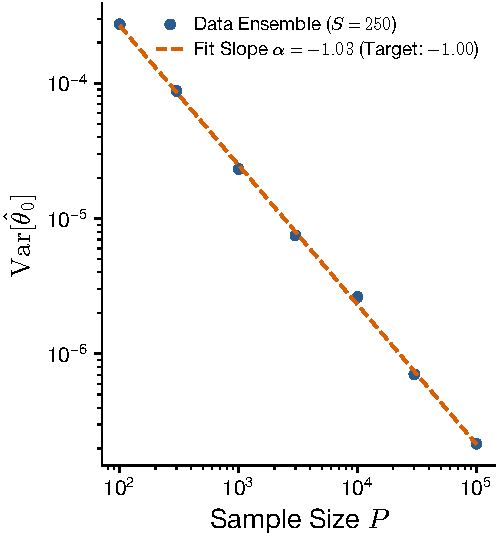
\includegraphics[width=\textwidth]{figures/clt_verification_variance_vs_P.pdf}
        \label{}
        \caption{}
    \end{subfigure}
    \hfill
    \begin{subfigure}{0.4\textwidth}
        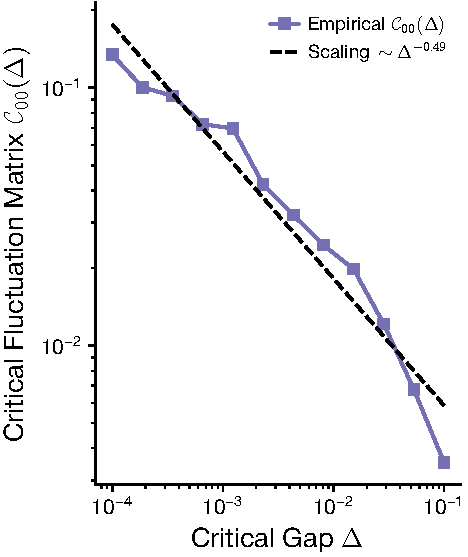
\includegraphics[width=\textwidth]{figures/noise_gap_scaling_C00_vs_Delta.pdf}
        \label{}
        \caption{}
    \end{subfigure}
    \label{}
    \caption{\textbf{Validation of Central Limit Theorem scaling and gap-dependent fluctuation amplification for finite sample size $P$.}
    \textbf{(a)} Variance of the estimated parameter $\operatorname{Var}[\hat{\theta}_0]$ versus dataset size $P$ over $S = 250$ independent data realizations. The empirical slope $\alpha = -1.03$ confirms the standard $O(P^{-1})$ CLT decay of estimator variance (Eq. 54).
    \textbf{(b)} Scaling of the empirical covariance matrix entry $\mathcal{C}_{00}(\Delta)$ with critical gap $\Delta$. The power-law scaling $\mathcal{C}_{00}(\Delta) \sim \Delta^{-0.49}$ highlights the noise amplification driven by the ill-conditioning of the empirical design matrix $\hat{M}$ as $\Delta \to 0$.}
\end{figure}


\section{Finite Sampling with noisy target}
$$r_\mu \overset{i.i.d}{\sim} \rho_\Delta, $$
$$ y = g(r_\mu) + \xi_\mu; \hspace{1em} \xi \sim \mathcal{N}(0,\tau^2),$$
and
$$\phi(r) = (1, r, r^2,..., r^{K-1})^T$$
\end{document}
